            \vspace{-5mm}
    \subsection*{Extra Experiment 2 : SDN-based Application-aware Routing for App Y}
        \subsubsection*{The Path, Flow Table}
            포트간에 설정된 delay와 대역폭을 고려하여 Application Y의 condition 을 만족하는 아래의 path를 찾았다.\\
                \vspace{-4mm}
            \begin{figure}[!h]\centering 
            	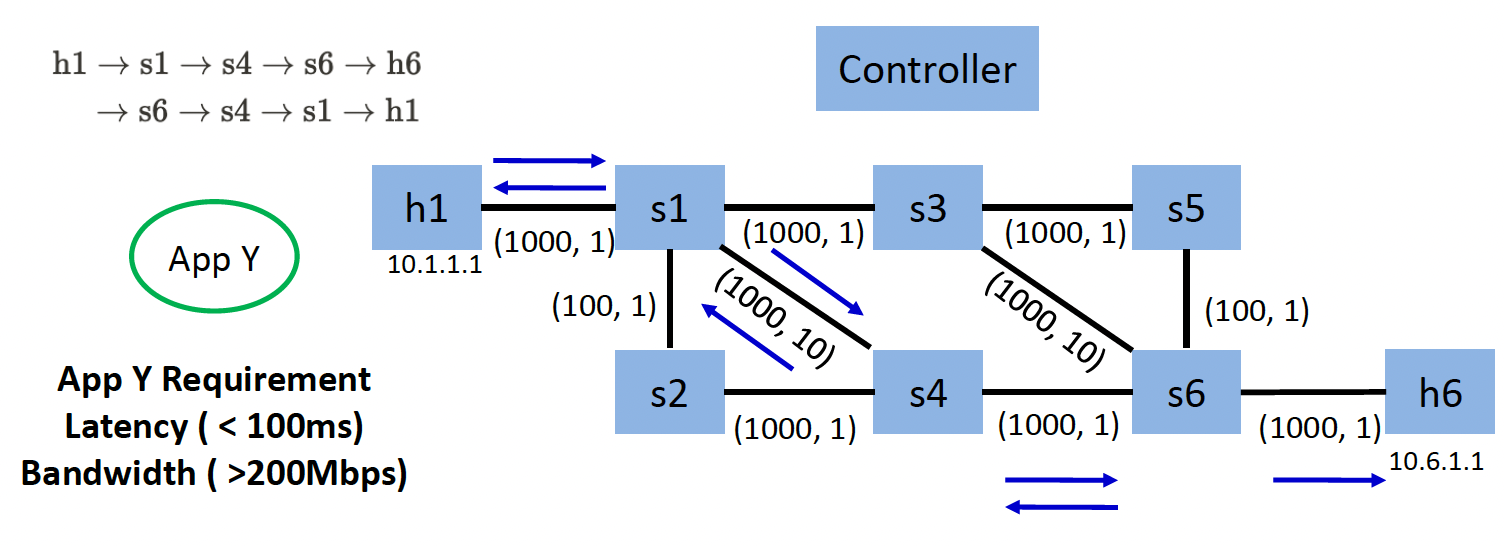
\includegraphics[width=.7\textwidth]{image/week08/e2-0.png}
            	\caption{\footnotesize
            	 Application Y의 requirement 를 만족시키는  Routing Path}
            	\vspace{-10pt}
            \end{figure}
            
            해당 path를 따르게 하기위해서 flow table에 다음의 command로 flow를 추가해 주었다.
            \begin{listing}[h!]
            \inputminted[framerule = 1pt,framesep = 2mm , frame = lines, fontsize=\footnotesize]{python}{./code/week08/flow-e2.sh}
            % \vspace{-5mm}
            \vspace{-4mm}
            \caption{\footnotesize Extra experiment 2's dpctl flow-add commands}
            \end{listing}
            
            \vspace{-2mm}
            추가된 flow들의 flow table은 아래와 같다.\\
                \vspace{-4mm}
            \begin{figure}[!h]\centering 
            	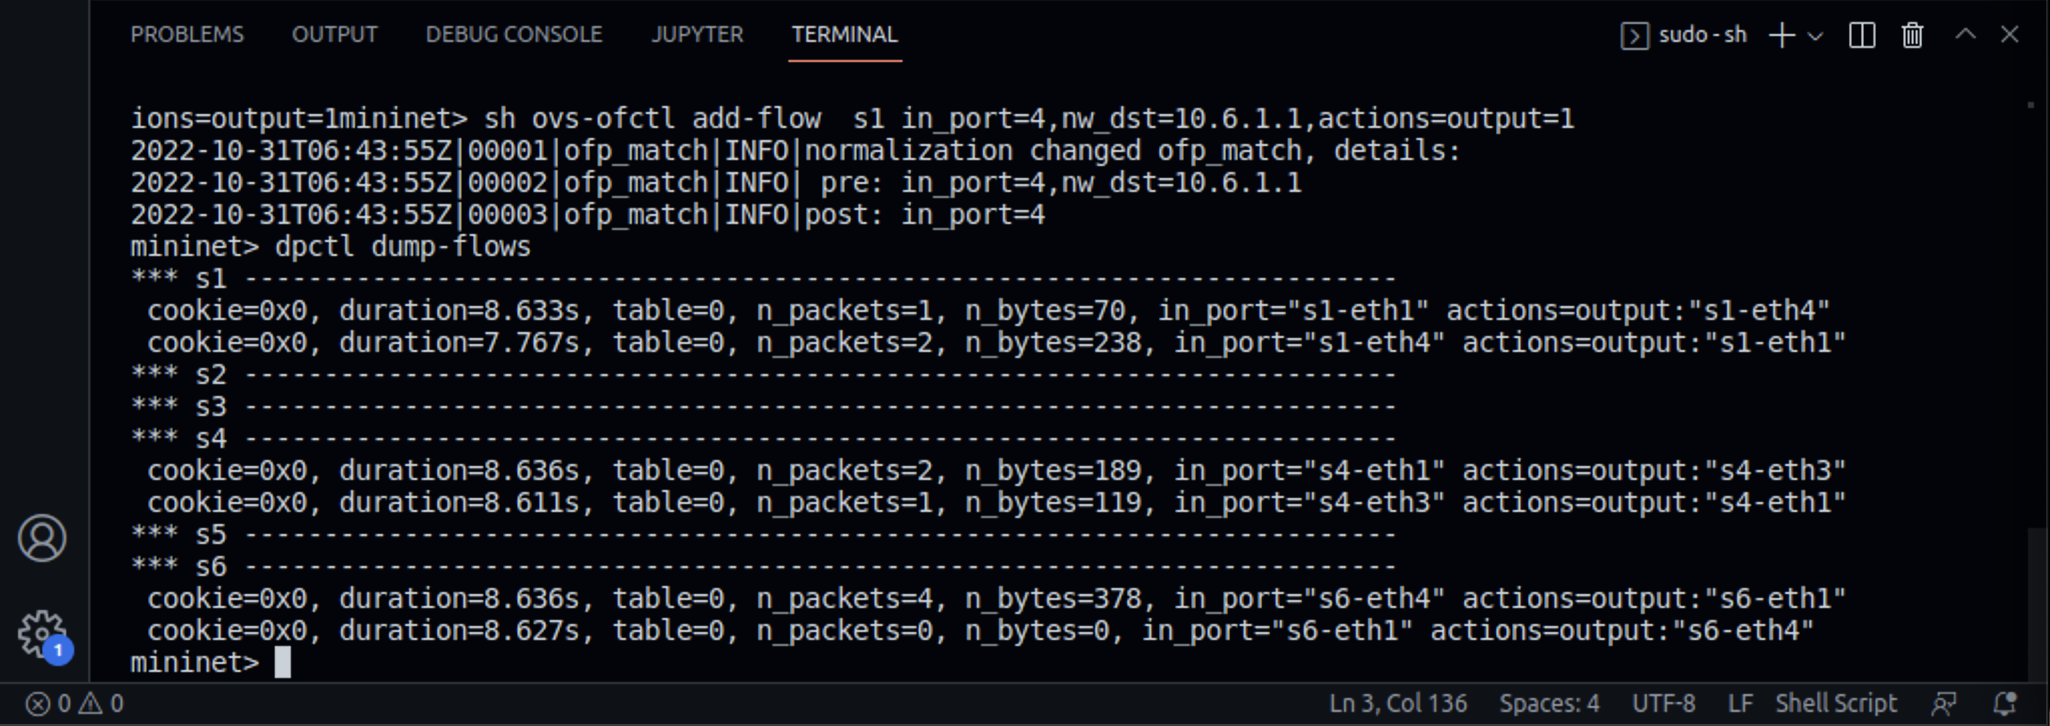
\includegraphics[width=.99\textwidth]{image/week08/e2-1.png}
            	\caption{\footnotesize
            	 Extra experiment 2's flow table}
            	\vspace{-10pt}
            \end{figure}
            % \clearpage
%---------------------------------------------------------------------------------%
        \subsubsection*{Ping Table : Latency}
        \begin{equation*}
            \text{Latency} \simeq 0.5 \times \text{Round Trip Time} \quad \Rightarrow 0.5 \times 27.017 = 13.508 ms\ \leq\ 100 ms \to \text{ Y application's latency}
        \end{equation*}
            \vspace{-4mm}
        \begin{figure}[!h]\centering 
        	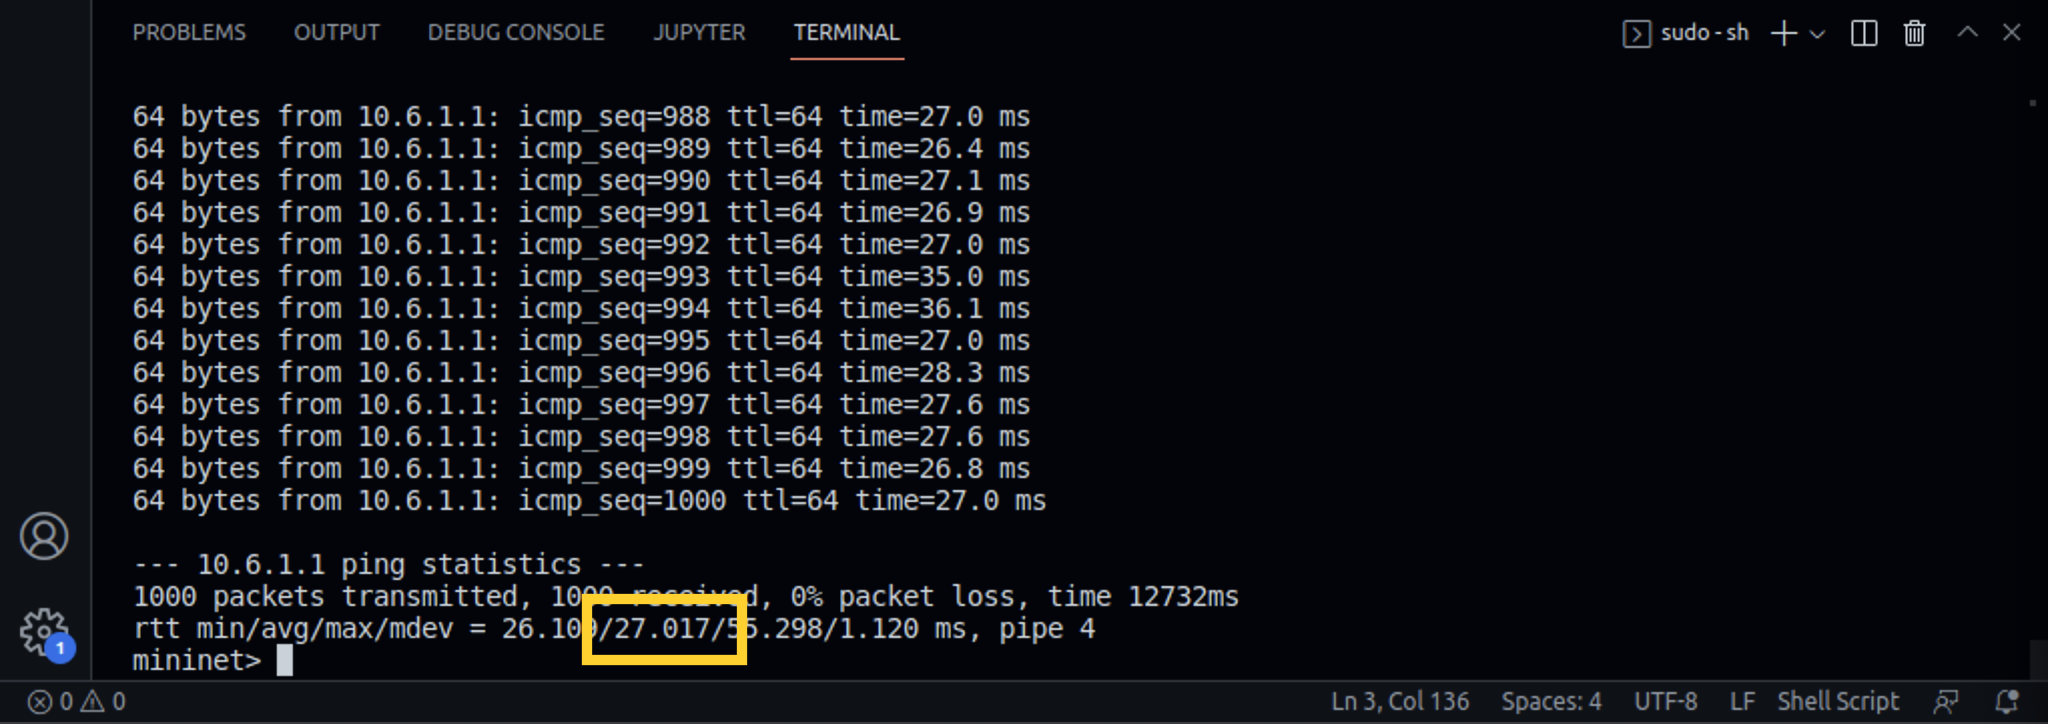
\includegraphics[width=.99\textwidth]{image/week08/e2-2.png}
        	\caption{\footnotesize
        	 Extra experiment 2's pingtest results value of RTT, $27.017\ ms$ average}
        	\vspace{-10pt}
        \end{figure}
        \subsubsection*{ipref Test : Bandwidth}
        대역폭이 900 Mbps 와 906 Mbps 로  대역폭 기준 인 200 Mbps를 크게 상회하는 결과를 확인할 수 있다. \\
\clearpage
        \begin{figure}[!h]\centering 
        	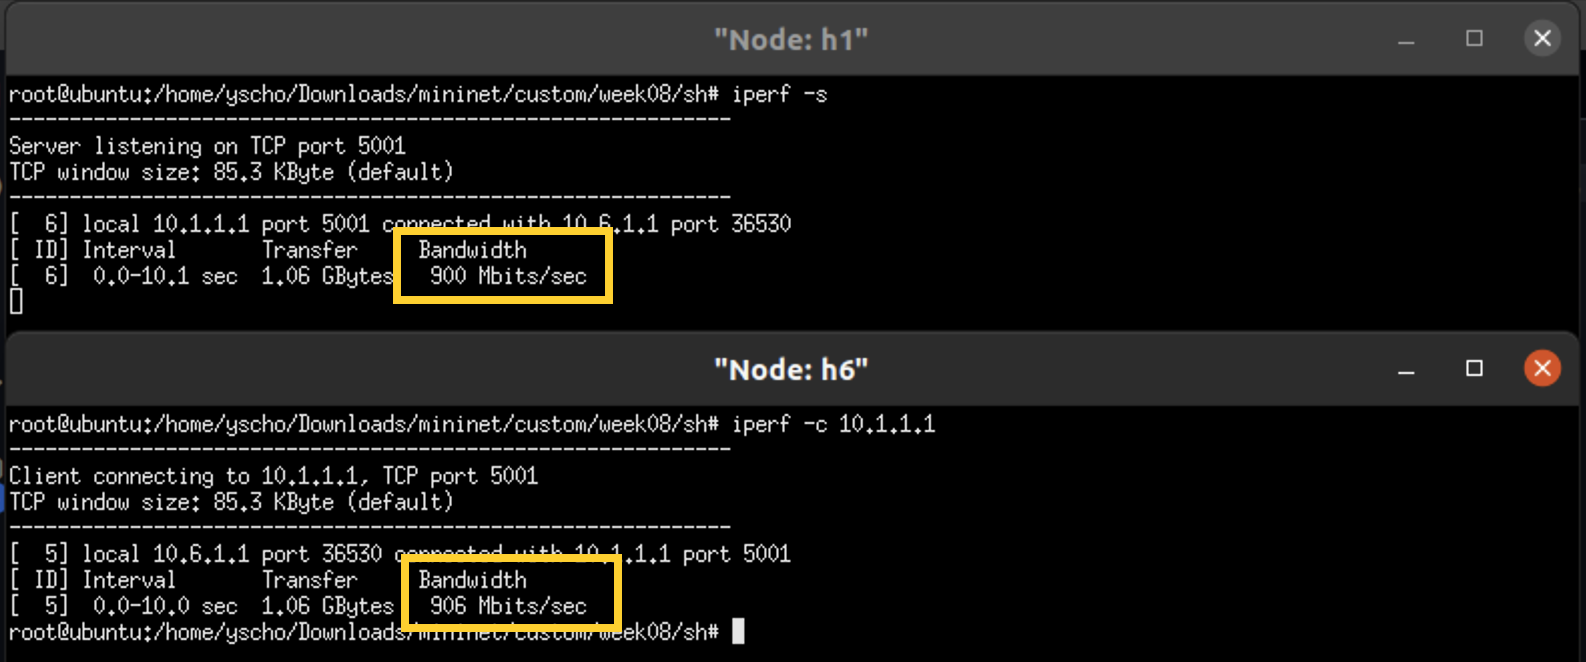
\includegraphics[width=.99\textwidth]{image/week08/e2-3.png}
        	\caption{\footnotesize
        	 Experiment2's the measured bandwidth value of host h1\& h6, 900 Mbits/sec 906Mbits/sec }
        	\vspace{-10pt}
        \end{figure}
\clearpage
%---------------------------------------------------------------------------------%